\documentclass[preprint]{aastex}
\usepackage{amsmath,amssymb}
\usepackage{mathrsfs}
\usepackage{graphicx}
\usepackage{natbib}
\bibliographystyle{apj}

\newcommand{\mli}[1]{\mathit{#1}}
%\usepackage{epstopdf}

\begin{document}

\title{Type Ia Supernova Model}
\author{Alex Kim}

\section{Model}
We infer a Hubble diagram based on measurements of discovered transients
classified as Type~Ia supernovae (SNe~Ia).  The inferred Hubble diagram can be
expressed as
\begin{equation}
P(\vec{\mu},\vec{z}| \vec{\hat{D}}=1, \vec{\hat{ADU}}, \vec{\hat{T}}_S=\text{SN~Ia},\vec{\hat{z}}_S,
\vec{\hat{\theta}}_S,\vec{\hat{z}}_H,\vec{\hat{\theta}}_H),
\label{hd:eqn}
\end{equation}
where the inferred quantities are the set of distance moduli ($\vec{\mu}$)
and redshifts ($\vec{z}$), and 
the measurements include: $\hat{D}$ the boolean that indicates that
the transient was discovered; $\hat{ADU}$ the transient photometry;
spectroscopically derived transient
typing, redshift and parameters $\hat{T}_S$, $\hat{z}_S$, $\hat{\theta}_S$;
and the redshift and parameters of the associated host galaxy $\hat{z}_{H}$, $\hat{\theta}_H$.
The conditions $\vec{\hat{D}}=1$, $\vec{\hat{T}}_S,=\text{SN~Ia}$ hold as only transients
discovered and classified as SNe~Ia are modelled.  We use the convention of using carets $\hat{}$
to  label measurements. 

A sketch of a model explaining the data is depicted through the Probabilistic Graphical Model
(PGM)
shown in Figure~\ref{pgm:fig}.
Although only transients that are detected and classified as
SN~Ia are modeled, the model accommodates the possibility that they could not have been found
or not classified as SN~Ia.

\begin{figure}[htbp] %  figure placement: here, top, bottom, or page
   \centering
   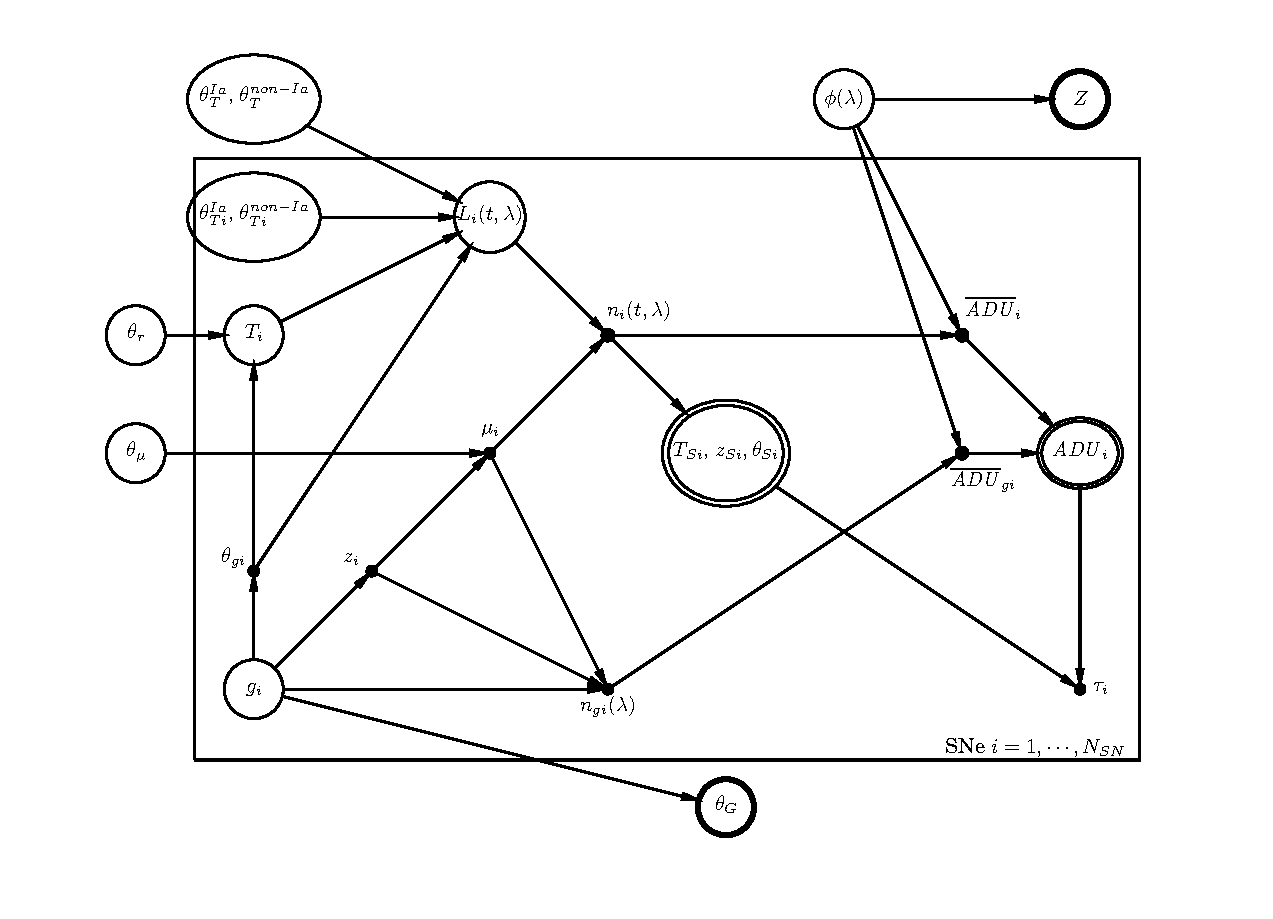
\includegraphics[width=7in]{/Users/akim/project/abc/results/hdpgm.eps} 
   \caption{Probabilistic Graphical Model for the SN~Ia analysis.
   The bottom right corner containing the connection between observed light curves
   $\hat{f}$, transient spectral information $\hat{z}_S$, $\hat{\theta}_S$, and
   host information $\hat{z}_H$, $\hat{\theta}_H$ with the determined type, redshift, and distance
   modulus $\hat{T}$, $\hat{z}$, and $\hat{\mu}$ is the purview of
   the traditional light-curve and Hubble diagram fitters.
   \label{pgm:fig}}
\end{figure}

One feature to note is that $\mu$ is a model parameter; most analyses instead
directly have cosmological parameters $\{\Omega_M, \Omega_\Lambda, w_0, w_a\}$.
A motivation is to provide results that can be applied to test arbitrary cosmological models:
indeed the model-dependence of the $\mu$'s reported for high-$z$ supernovae 
\citep[e.g.][]{2012ApJ...746...85S} is a source of confusion to the community.
An example of a non-parametric model for $\mu$ that is independent of cosmological
parameters is given in the Appendix of
\citet{2013ApJ...764..116W}.

\subsection{Forward Model}
I first walk through the PGM as a forward process.  This is useful for understanding
how the model would be simulated.

Discovered transients typed as SNe~Ia are modeled.  Each has
a cosmological redshift and corresponding distance modulus; these $z$-$\mu$ pairs are the  parameters that
constitute the Hubble diagram.  For the moment, the coordinates RA/Dec are considered
precisely determined from the images.

Each transient indexed by $i$ is of a certain type $T$ and comes from a  host galaxy of type $G$.  
(``Host'' includes the host as well as  all galaxies that project onto the coordinate of
the transient.)  The
transients (galaxies) are modeled and described by global parameters $\theta_T$ ($\theta_G$),
and  parameters specific to the transient $\theta_{Ti}$ ($\theta_{Gi}$).  For example, the SALT2 SN~Ia
model has individual $c$ and $x_1$ parameters that would fill $\theta_{Ti}$,
and global $\alpha$, $\beta$, and intrinsic dispersion  parameters  common to all supernovae
 and  underlying  $c$ and $x_1$ distributions that would fill $\theta_T$.
The Type model includes  information on the
source and line-of-sight effects, which specify the effective SED. 
This SED, redshift, and  distance modulus determine the photon flux incident above the Earth's
atmosphere, $n$ and $n_g$.  

The experiment has an optical chain summarized by the transmission functions $\phi(\lambda)$, which determine the expected counts of the transient and galaxy, $\mathit{ADU}$ and
$\mathit{ADU}_g$.   These expected counts in turn determine realized  transient counts 
$\mathit{ADU}_V$.
The signal to noise of the realized counts specify the probability of discovery
$\hat{D}$ .    The photometry of the subset of discovered transients
are denoted as $\hat{\mathit{ADU}}$.

For discovered transients, there may be spectra of the object itself
from which typing, redshift and spectral parameters $\hat{T}_S$, $\hat{z}_S$, $\hat{\theta}_S$ are derived.
From amongst the detected galaxies $\hat{\mathit{Gals.}}$  a host is associated with the transient
based on its RA/Dec, its
host redshift (spectroscopic or photometric) and parameters are $\hat{z}_{H}$, $\hat{\theta}_H$.

The observatory transmission $\phi$ are calibrated $\hat{Z}$.


\subsection{Backward Model}
 
I now systematically
examine the model going backwards, from the observables to the fundamental parameters.
This is useful for understanding dependencies in constructing the likelihood.

The observables are:
\begin{description}
\item[$\hat{\mathit{Gals}}$] Detected galaxies from which a host is associated with a transient.
Depends on the model for galaxies $\theta_G$.
\item[$\hat{D}$] Transient detection.  It depends on
the realized signal $\hat{\mathit{ADU}_V}$ and its noise, mostly through the signal-to-noise
$\mathit{SNR}$.
\item[$\hat{\mathit{ADU}}$]  Photometry of discovered transients.  Exactly the value
of the  realized signal $\mathit{ADU}_V$ and discovery $\hat{D}$.
\item[$\hat{z}_H$, $\hat{\theta}_H$] Host galaxy redshift and properties from spectroscopic
and photometric data, based on association
of the host from the pool of detected galaxies $\hat{\mathit{Gals}}$ and the transient RA/Dec.
\item[$\hat{T}_S$, $\hat{z}_S$, $\hat{\theta}_S$] Transient redshift and properties from
spectroscopic data. I skip the details of the actual measurement  and make a direct association
with the fluxes of the transient and underlying galaxy $n$, $n_g$.
\item[$\hat{Z}$] Calibration zeropoints.  Depends on the calibration process
and the underlying transmission functions $\phi(\lambda)$.  This may be a zeropoint
but most probably will be calibrated transmission functions.
\end{description}

The following are elements of the model.
\begin{description}
\item[$\mathit{ADU}_V$]  Realized counts
of the transient.  Depends
on the expected counts of the transient and host $\mathit{ADU}$, $\mathit{ADU}_g$.
This is distinct from $\hat{\mathit{ADU}}$, which only has photometry of detected transients.
\item[$\mathit{ADU}$, $\mathit{ADU}_{g}$]  Expected counts
of the transient and background galaxy respectively.  Depends
on the incident fluxes $n$, $n_g$ and the instrumental
transmission $\phi(\lambda)$.
\item[$\phi(\lambda)$] DES transmission functions.
\item[$n$, $n_g$] The incident fluxes at Earth of the transient and background
galaxy.  Depends on  $z$ and $\mu$, and the SEDs of the Type and Host as
specified by $\theta_{Ti}$, $\theta_{Gi}$,$\theta_{T}$, $\theta_{G}$.
\item[$\theta_{Ti}$, $\theta_{Gi}$] Parameters that describe the properties of the individual transient
and host respectively.
\item[$\theta_{T}$, $\theta_{G}$] Parameters that describe the global properties of the transient
and host models.
\item[$T$,$G$]  The type of transient and projected galaxies (referred to as host), which
specifies which model to use. The realization depends on the redshift $z$.
\item[$\vec{\mu}$, $\vec{z}$]  The true distance moduli and cosmological redshifts under
consideration.  Each redshift has a unique distance modulus.
\item[$\mathbf{RA/Dec}$] The coordinate of the transient.  It will be the actual coordinate of the found discovered object.
\end{description}

\section{Subsections of the Model}

\subsection{Type}
\label{type:sec}
Given that our transient sample may not consist purely of SNe~Ia, the model
has a term of the form $P(T, G | z,\mu)$, which should account for all types of
objects that could potentially be mistaken for Type~Ia:
the rates and association with host galaxies are described for
the full population of potential interlopers.
%Note the condition $\hat{T}=\text{SN~Ia}$ means that non-Ia transients unlikely to
%be identified as SN~Ia can be described with poorer accuracy.
This term is not currently well known, particularly at the highest redshifts probed by DES.
It could be constructed through modeling, although then the uncertainties 
of that modeling must in turn be quantified.

I posit that a concise way of addressing this term is to only model $T=\text{SN~Ia}$,
and experimentally determine $P(\text{non-Ia})$, 
$\left. \langle \mu-\mu_{model} \rangle \right|_{non-Ia}$, and its uncertainty for the
sample of non-Ia's that are discovered and misclassified as SN~Ia.
This measurement is achieved through spectroscopic
typing of a subset drawn from the populations used in the Hubble diagram.
Other supernova surveys
with spectroscopic follow-up (e.g.\ SNLS) that replicate the DES population
can be used, for example on magnitude-limited samples with
complete  spectroscopic follow-up. 
The weighted bias would be added as a correction to the Hubble diagram under the assumption that all objects are SNe~Ia.

To minimize the contribution of non-Ia contamination we strive for
an excellent classifier so that $P(non-Ia) \rightarrow 0$.


\subsection{Host Matching}
\sloppy
The host-galaxy properties depends on the galaxy catalog and the transient
coordinates $P(\hat{z}_H, \hat{\theta}_H | \hat{\mathit{Gals.}}, \text{RA/Dec})$.  With a
spectrum of the transient and the underlying background, identification of the host galaxy
is usually straightforward.
Otherwise, projections or ambiguous cases can result in the misidentification of
the host.

A similar strategy can be taken as with non-Ia contamination in \S\ref{type:sec}:
analyze the supernova assuming a correct host match, and
experimentally determine $P(\text{mismatch} )$ and
$\left. \langle \hat{\mu}-\mu(z)\rangle \right|_{\text{mismatch}}$, $\left. \langle \hat{z}-z \rangle \right|_{\text{mismatch}}$ to correct bias in the Hubble diagram. 
We strive to have $P(\text{mismatch}) \rightarrow 0$.


\subsection{Type~Ia Supernova Model}
\label{snmodel:sec}
The model contains a piece $P(\hat{\mathit{ADU}}_{i} \hat{z}_{Si}| \mu_i,z_i,\theta_T, \theta_{Ti}, ,\phi(\lambda))$, which
is the piece that describes underlying SN~Ia properties and light-curve fits.

Need something more general?
$P(\hat{D}_i,\hat{\mathit{ADU}}_{i}, \hat{T}_{Si}, \hat{z}_{Si}, \hat{\theta}_{Si}, \hat{z}_{Hi}, \hat{\theta}_{Hi}
 | \mu_i,z_i,T_i,\theta_T,\theta_{Ti},\phi(\lambda))$
\subsection{Detection Efficiency}
There term $P(\hat{D}|\mathit{ADU}_V)$.  For all high-redshift supernova searches
I know of, this depends on the signal-to-noise of the data, and very weakly on the
structure of the underlying galaxy.  Our detection is now based on machine learning,
we should confirm that detection dependencies do not depend on our model parameters
(except for RA/Dec).

\section{Systematic Tests}
The Hubble diagrams of subsets of data quantify systematic uncertainty.  
Subsets that may be expected to show evidence for systematics include:
spectroscopically typed SNe~Ia; transients in deep (3) versus shallow (1/2) DES fields;
transients with NIR data; splits based on host properties.

A potentially more probative test is to compare the distance moduii inferred for the same
supernovae, but reducing the amount of data considered.  A subset of DES
transients have higher signal-to-noise, spectroscopic confirmation, and NIR coverage than
the average transient, we can take away that extra information in calculating distance modulus
to get $P(\mu | \mathit{data} - \mu | \mathit{data}^-, z | \mathit{data} - z | \mathit{data}^-)$.
It is possible that differences in $\mu$s and $z$s have smaller uncertainties that the
$\mu$ and $z$ alone due to common measurement uncertainties. 

\bibliography{/Users/akim/Documents/alex}

\end{document}

